\documentclass{article}

\usepackage{url}
\usepackage{microtype}
% \usepackage{fullpage}
\usepackage{graphicx}
\usepackage{subcaption}

\begin{document}

\begin{centering}
  \Large{\textbf {Intrigue}} (v0.1)\\
  A Game for Three Royal Advisors\\
\end{centering}

\vspace{0.5cm}

{\itshape The King has died under mysterious circumstances. The
  kingdom is in tumult as different factions maneuver their preferred
  person toward the empty throne.  Whoever is selected will have a
  tenuous grasp on the reins of the kingdom and may not survive long.

  But you will be perfectly safe. You are one of the advisors---the force
  behind the throne. By manipulating the relationships among the
  various potential rulers, you can ensure that your favored
  choice comes out on top.
}

\vspace{0.5cm}

Thank you for downloading \textit{Intrigue}. Please feel free to reach
out to me with feedback from your experience through email to
\url{pvgestwicki@bsu.edu}. 


\section*{Preparation}

You will need some tokens for keeping track of score. Coins or chits from
another game will work fine.

Print all the card and token sheets. All are single-sided except
the small cards marked \textit{Favor}. These can be printed duplex or
combined in a sleeve; there should be an A-B-C set for each of player
numbers 1, 2, and 3. The larger cards are designed so that you can
use penny-sleeves and poker cards to back them for ease of shuffling
and play.


\section*{Setting Up}

Separate the \textit{Character} cards from the other cards.
Shuffle these and put three randomly into play, forming a circle.
These are the characters who are vying for the throne.

Place a Character Token arbitrarily on each character, marking them
as character A, B, or C, then place a ``+3'' and ``+1'' support
token on each character.

Shuffle the remaining cards to form the draw deck. These consist of
\textit{Action}, \textit{Support}, and \textit{Relationship} cards.

Give each player three points and a set of three Favor cards. For example,
Player 1 will have the three A, B, and C cards that have the number ``1''
on the back.

Choose a starting player using your favored method and begin the first round.

\begin{figure}
  \centering
  \begin{subfigure}{0.5\textwidth}
    \centering
    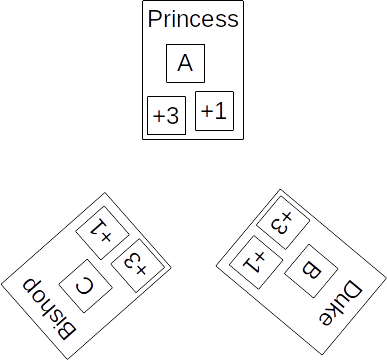
\includegraphics[width=2in]{layout_initial}
  \end{subfigure}%
  \begin{subfigure}{0.5\textwidth}
    \centering
    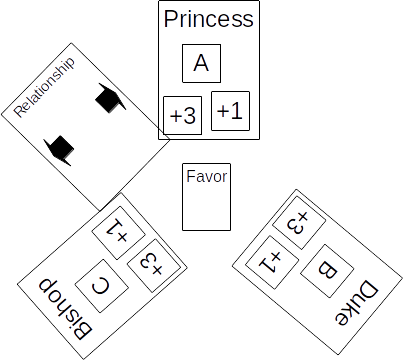
\includegraphics[width=2in]{layout_after}
  \end{subfigure}
  \caption{The initial character layout (left) and the positioning
     of a relationship and the favor cards (right).}
\end{figure}


\section*{Playing the Game}

During each round, characters are competing to earn support from
different parts of the kingdom, while the players are positioning
themselves to be the strongest public supporter of the one who comes
out on top.

Each player takes a turn, and then play passes to the left.
On a player's turn, they may do one of the following:
\begin{itemize}
\item Take a support token from a character. 
\item Play a card from their hand.
\item Play a Favor card face-down in the center of the table.
\end{itemize}

There are three types of cards that a player may have drawn from the
deck: \textit{Action}, \textit{Support}, or \textit{Relationship}.
Any of these can be played face-down in the support stack behind a
character, which means that the card's support value---shown in the
bottom center of the card---will contribute to that character.
Normally, when you play a card in this manner, its text is ignored;
however, some
\textit{Support} cards additionally allow you to play them face-up in
order to trigger other effects.

\textit{Action} cards are played, resolved, and discarded.

\textit{Relationship} cards are played between characters so that their
arrows point unambiguously to two characters. There can only ever
be one relationship between two characters. A new relationship can be
played to replace an old one but only if one is positive and the
other is negative. (Remember: zero is neither positive nor negative.)

\subsection*{End of Round}

The round continues until one player has no cards, at which point
the round is over.

First, reveal all support cards that were played for each character.
Determine each character's total support value by adding the
values on these cards as well as any relationships in play.
Remember that the value for some support cards may depend on
traits that the character has: if the character has a listed trait,
use the value left of the slash, and if a character does not, use
the lower value on the right.
The winner of the round is the character with the highest support
value unless this is overridden by a relationship in play.
In the case of a tie, compare the Priority numbers on the
tied characters, which are shown on their character cards:
the higher priority breaks the tie.
Place one point token on the winning character.

Now, determine how many points were earned by the players.
A player who has support tokens for the winning character
gains the number of points shown on the token. Then, players
lose one point for each support token of a non-winning character.

The game is over after three rounds or if any player has
zero points; move to the end of game instructions.
Otherwise, set up for the next round by completing the following steps:
\begin{itemize}
\item Return support tokens to the characters.
\item Collect all the cards in characters' support stacks and the
  discard pile and shuffle these into the draw deck.
\end{itemize}

Note that you do not collect played relationship cards nor do you
collect the favor cards; those all stay in play for the next round.

\subsection*{End of Game}

The character with the most point tokens ascends to the throne.
Break ties using the Priority values as described above.

Flip over the stack of played Favor cards, allowing you to proceed
through them in the order they were played.  The first player to have
gained favor with the new monarch gains a three point bonus; each
subsequent player gains one point.  Players lose one point for each
favor they played of a losing character.

The player with the most points at the end of the game is victorious.
They have positioned themselves to be the real power in the kingdom.
Victory is shared in the case of a tie.

\end{document}
